% senior_thesis-proposal.tex
% Gregory M. Kapfhammer
% CMPSC 580, Spring 2013
%
% Revised by R. Roos
% Sep 2013
%
% This document provides a sample senior thesis proposal template for use
% by students in Allegheny's CS and Applied Computing programs.
%
%   *******************************************************************
%   * LOOK FOR BLOCK COMMENTS SUCH AS THIS ONE FOR AN EXPLANATION OF  *
%   * THIS DOCUMENT AND HOW TO MODIFY IT FOR YOUR OWN PROPOSAL!       *
%   *                                                                 *
%   * ANY LINE BEGINNING WITH A "%" IS A LATEX COMMENT AND IS IGNORED *
%   * BY THE LATEX PROCESSOR. YOU ARE ENCOURAGED TO COMMENT YOUR OWN  *
%   * LATEX CODE.                                                     *
%   *******************************************************************

%   ********************************************************************
%   * THE FIRST SECTION OF THE LATEX FILE IS THE "PREAMBLE." IT        *
%   * INSTRUCTS LATEX TO IMPORT SPECIAL PACKAGES FOR THINGS LIKE       *
%   * INCLUDING FIGURES, DOUBLE-SPACING, COLORED TEXT, ETC.            *
%   * DEPENDING ON YOUR NEEDS, YOU MAY FIND IT NECESSARY TO USE PACK-  *
%   * AGES THAT ARE NOT INCLUDED IN THIS TEMPLATE. SIMPLY IMITATE THE  *
%   * "\usepackage{...}" COMMANDS SHOWN BELOW.                         *
%   ********************************************************************

%   ********************************************************************
%   * BEGINNING OF PREAMBLE:                                           *
%   ********************************************************************
\documentclass[11pt]{article}

\usepackage[T1]{fontenc}
\usepackage{mathptmx}
\topmargin 0.0in
\setlength{\textwidth} {420pt}
\setlength{\textheight} {620pt} 
\setlength{\oddsidemargin} {20pt}
\setlength{\marginparwidth} {72in}

%   ********************************************************************
%   * Many of the commands below were simply copied over from an older *
%   * version of the proposal template; you can just leave them as     *
%   * they are (or you can delve into the TeX/LaTeX documentation      *
%   * and figure out what they do). Otherwise, jump ahead to the next  *
%   * block of comments, where you will enter title, abstract, etc.    *
%   ********************************************************************

\usepackage{fancyhdr} 
\usepackage{url}
\usepackage{graphicx}
\usepackage{setspace}

% set it so that subsubsections have numbers and they
% are displayed in the TOC (maybe hard to read, might want to disable)

\setcounter{secnumdepth}{3}
\setcounter{tocdepth}{3}

% define widow protection

\def\widow#1{\vskip #1\vbadness10000\penalty-200\vskip-#1}

\clubpenalty=10000  % Don't allow orphans
\widowpenalty=10000 % Don't allow widows

% this should give me the ability to use some math symbols that 
% were available by default in standard latex (i.e. \Box)

\usepackage{latexsym}

% define a little section heading that doesn't go with any number

\def\littlesection#1{
\widow{2cm}
\vskip 0.5cm
\noindent{\bf #1}
\vskip 0.0001cm 
}

\pagestyle{fancyplain}

\newcommand{\tstamp}{\today}   
\renewcommand{\sectionmark}[1]{\markright{#1}}
\lhead[\Section \thesection]            {\fancyplain{}{\rightmark}}
\chead[\fancyplain{}{}]                 {\fancyplain{}{}}
\rhead[\fancyplain{}{\rightmark}]       {\fancyplain{}{\thepage}}
\cfoot[\fancyplain{\thepage}{}]         {\fancyplain{\thepage}{}}

\newlength{\myVSpace}% the height of the box
\setlength{\myVSpace}{1ex}% the default, 
\newcommand\xstrut{\raisebox{-.5\myVSpace}% symmetric behaviour, 
  {\rule{0pt}{\myVSpace}}%
}

% leave things with no spacing extra spacing in the final version of the paper
\renewcommand{\baselinestretch}{1.0}    % must go before the begin of doc

% suppress the use of indentation for a paragraph

\setlength{\parindent}{0.0in}
\setlength{\parskip}{0.1in}

\begin{document}

\doublespacing

% handle widows appropriately
\def\widow#1{\vskip #1\vbadness10000\penalty-200\vskip-#1}

% build the title section

\makeatletter

\def\maketitle{%
  %\null
  \thispagestyle{empty}%
  %\vfill
  \begin{center}%\leavevmode
    %\normalfont
    {\Huge \@title\par}%
    %\hrulefill\par
    {\normalsize \@author\par}%
    \vskip .4in
%    {\Large \@date\par}%
  \end{center}%
  %\vfill
  %\null
  %\cleardoublepage

  }

\makeatother

%   ********************************************************************
%   * Here is the first place where you need to begin customizing:     *
%   * Enter you name, the title of your proposal, etc., in the places  *
%   * indicated by the comment "% CHANGE!".                            *
%   ********************************************************************

\vspace*{-1.1in}
\title{Computer Science 220 Final Report}  % CHANGE!

% build the author section
\author{
        Andreas Landgrebe\\  % CHANGE!
        Computer Science 220 \\
        Department of Computer Science\\
        Allegheny College \\
        {\tt landgrebea@allegheny.edu}  \\  % CHANGE!		
        \vspace*{.1in} \today \\ \vspace*{.1in}
}

\maketitle       % use the default title stuff

% Default "abstract" environment is too small; customize one instead:
%\begin{center}
%\large\bf Abstract
%\vspace{-1em}  % Reduce space between header and the abstract
%\end{center}

%   ********************************************************************
%   * Here is the second place where you need to customize:            *
%   * enter your abstract in the "quote" environment:                 *
%   ********************************************************************

%\begin{quote}
%Provide a concise summary of your proposed research. Remember that
%the abstract is {\it not} an introduction, it is a {\it summary} of the
%entire document. It makes sense to wait to write the abstract until the
%rest of the document has been written.
%\end{quote}

\vspace*{-.4in}
\section{Background}
\label{sec:background}
\vspace*{-.1in}
%Give some brief background (who created it? when? why?)
The programming language that I had studied throughout the final project was Swift. Swift was created by Chris Lattner and Apple Inc. Chris Lattner started to development of the Swift programming language in 2010 along with many other programmers at Apple. This programming language took language ideas from many other lanauges such as Objective-C, Rust, Haskell, Ruby, Python, C\# and many others. The first release of Swift appeared on June 2, 2014. It has since then been upgraded and on December 1, 2015, version 2.2 was made open srouce and has made available now for Apples's and Linux's platforms. The Swift programming lanauage was developed because Apple wanted to to create a programmiung language that is a easier to use instead of using Objecitve-C. There are many reasons to choose to learn Swift rather than learning and using Objective-C. One of the main reasons is that Swift is much more human readable than Objective-C. 

\vspace*{-.4in}
\section{Importance}
\label{sec:importance}
\vspace*{-.1in}
%Explain its importance (where is it used? why is it worth studying?)
The Swift Programming language is used for iOS, OS X, watchOS and tvOS development. The primary use of the Swift programming language is the development of products created by Apple. It is worth studying due to the fact that this is the language being used in the future for development for Apple software. As of right now, the most popular Integreated Development Environment being used when writting Swift is Xcode. As of right now, Xcode is the only Integreated Development Environment being able to emulate and produce iPhone, iPad, iPod Touch, and Mac OS X applications. If one were to ever get involved in iOS mobile applications development and OS X development, then the best language that one would use would be Swift. One could have also used Objective-C but there are many reasons why one would use Swift compared to Objective-C.


\vspace*{-.4in}
\section{Similarity}
\label{sec:similarity}
\vspace*{-.1in}
%Compare to other languages. In what ways is it similar to them? What distinguishes it from similar languages?

Compared to other languages, there is will only one programming language that can write for iOS and OS X programming and that is Objective-C. When choosing each of the two languages one should learn to write for iOS and OS X development, it would be Swift. There are many reasons why one would decide to learn Swift over Objective-C. Some of these reasons is that Swift is easier to read, swift is easier to maintain, Swift is safer, Swift is unified with memory management, Swift requires less code, Swift is faster, fewer namne collisions with open source projects, Swift supports dynamic libraries, Swift Playgrounds encourages interactive coding, and Swift is a future you can influence.  




\vspace*{-.4in}
\section{Classification of Criteria}
\label{sec:classificartionofcritiera}
\vspace*{-.1in}
%How is it classified according to the criteria we've looked at, such as
%-compiled? interpreted?
% paradigm (imperative? functional? object oriented? special purpose? ...)
% scoping (lexical? dynamic? block-level scoping? function-level scoping? ... )
% typing (statically typed? dynamically typed? ...)
% other critieria (for instance, parameter passing methods - by value? by reference? applicative/normal/%lazy order? ...)

This programming language of Swift was compiled. This means that Swift is a language where the implementations are general compilers and not interpreters. It is also a multi-paradigm language. This means that it is object-oriented, functional, Imperative, and block structured. When it is imperative, it means that it uses statements that change a program's state. When it is object-oriented, that menas that Swift is on the concept of objects which are data structures tht contains data, in the form of fields and code in the form of procedures which are known as methods. Functional is a style of building the structure and elements of computer programs which treat computation as the evaluation of math functions and changing data. When it is block-strucutred, it means that sections of code is written as section of code which is grouped together. These blocks consist of one of more declarations and statements.
One key feature of Swift is option types. This allos references or values to operate in a manner similar to a pattern in where a pointer may be a value or null. In Swift, the syntax for that would either be a ! or a ?.

Swift is also statically typed language. This is means with Swift consits of defining interfaces between different parts of a computer progran and then checking if parts have connections in a consistent way.

%   ********************************************************************
%   * Enter the text of your introductory section here.                *
%   ********************************************************************

%Provide an intuitive motivation for and introduction to your proposed
%senior thesis research.  Whenever possible, you should use one or more
%concrete examples and technical diagrams.

%\vspace*{-.1in}
%\section{Related Work}
%\label{sec:relatedwork}
%\vspace*{-.1in}

%   ********************************************************************
%   * Enter the text of your related work section here.                *
%   ********************************************************************

%Summarize the previously published papers and books that are related
%to your proposed research.  Whenever possible, you should compare and
%constrast your approach with the ones that have been discussed in the
%past.  As you describe your papers, please make sure that you cite
%them properly \cite{conrad-gecco-selection-study}.

%\vspace*{-.2in}
%\section{Method of Approach}
%\label{sec:method}
%\vspace*{-.1in}

%   ********************************************************************
%   * Enter the text of your method of approach section here.          *
%   ********************************************************************

%Use technical diagrams, equations, algorithms, and paragraphs of text
%to describe the research that you intend to complete. See the \LaTeX\ source
%file for the proposal to learn how Figure \ref{intro-fig1} and Table 
%\ref{intro-tab1} were included. Be sure to number all figures and tables and to
%explicitly refer to them in your text.

%\begin{figure}[htbp]
%\centering
%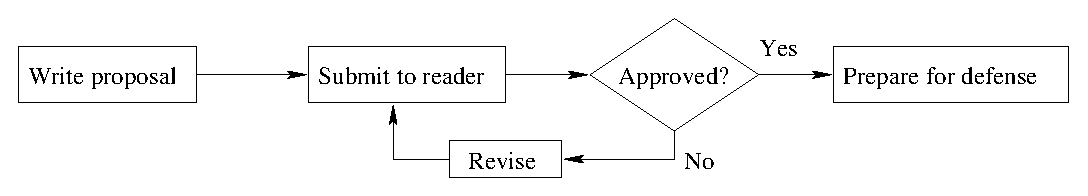
\includegraphics[width=5in]{flow}
%\caption{Flow graph for proposal-writing}
%\label{intro-fig1}
%\end{figure}

%\begin{table}[htbp]
%\centering
%\begin{tabular}{|c||c|c|}
%\hline
%\bf Task & \bf Begin Date & \bf End Date\\\hline\hline
%First draft & Now & 20 Sept\\\hline
%Second draft & 20 Sept & 27 Sept\\\hline
%Third draft & 27 Sept & 4 Oct\\\hline
%Fourth draft & 4 Oct & 11 Oct\\\hline
%Fifth draft & 11 Oct & 18 Oct\\\hline
%\end{tabular}
%\caption{Proposed work schedule}
%\label{intro-tab1}
%\end{table}

%\vspace*{-.2in}
%\section{Evaluation Strategy}
%\label{sec:evaluate}
%\vspace*{-.1in}

%   ********************************************************************
%   * Enter the text of your evaluation strategy section here.         *
%   ********************************************************************

%Explain what steps you will take to evaluate your proposed method.  If
%you intend to conduct experiments, then you must clearly define your
%evaluation metrics.

%\vspace*{-.1in}
%\section{Research Schedule}
%\label{sec:schedule}
%\vspace*{-.1in}

%Identify the main phases and tasks of your research project and set
%deadlines for when you will be able to complete each of these items.

%\vspace*{-.1in}
%\section{Conclusion}
%\label{sec:conclusion}
%\vspace*{-.1in}

%   ********************************************************************
%   * Enter the text of your concluding section section here.          *
%   ********************************************************************

%Provide a summary of your proposed research and suggest the impact
%that it may have on the discipline of computer science.  If possible,
%you may also suggest some areas for future research.



\nocite{*}

\bibliographystyle{plain}
\bibliography{report}

\end{document}

